\documentclass{ctexart}
\usepackage{graphicx}

\title{信息内容安全实验技术报告}
\author{ \\\\ 项目名称:微博的内容识别与控制\\\\ 韦昆杰  \\\\ 1181000420 \\\\  348971397@qq.com  \\\\\\\\\\\\\\\\\\\\\\\\\\\\}
\date{\today}

\graphicspath{{images/}}
\begin{document}
\maketitle
\newpage
\tableofcontents
\section{概述}
\subsection{测试目的}
对微博内容识别和控制进行测试,检查是否能完成预期功能,此外还有对性能的测试

\subsection{测试内容}

\begin{enumerate}
    \item 微博热搜子系统
    \item 微博搜索子系统
    \item 微博过滤子系统
    \item 微博管控子系统
    \item 数据库子系统
\end{enumerate}

\section{测试环境}
\subsection{硬件环境}
处理器:Intel(R) Core(TM) i5-8265U CPU @ 1.60GHz   1.80 GHz

内存:8.00 GB (7.85 GB usable)

System type	64-bit operating system, x64-based processor




\subsection{软件环境}
操作系统: Windows 10

IDE:Visual Studio Code

开发语言: TypeScript

界面实现: HTML CSS

数据库系统: MongoDB数据库


\section{测试方案}
\subsection{功能测试}
用户进入相应的功能页面,完成相应操作,实现对应功能
\subsubsection{微博热搜子系统}
用户在localhost:3000/trend网站点击热搜按钮,系统获取实时热搜并展示到网站页面上

\subsubsection{微博搜索子系统}
用户在localhost:3000/search网站输入要搜索的微博关键字并提交,系统获取对应的微博存储到数据库,并展示到网站页面上
\subsubsection{微博过滤子系统}
用户在localhost:3000/search网站输入要过滤的微博关键词,系统根据KMP或AC算法匹配微博,将匹配到的微博展示到网页页面上
\subsubsection{微博管控子系统}
用户在localhost:3000/control网站输入要管控的微博URL或在localhost:3000/search选择管控过滤的微博,系统将举报需要管控的微博
\subsubsection{数据库子系统}
用户可以在MongoDB数据库看到存储的热搜和微博
\subsection{性能测试}
测试BF、KMP、AC算法匹配相同字符串需要的时间

测试网页交互各项功能是否正常且流畅
\section{测试方法与结果分析}
\subsection{功能测试}
\subsubsection{微博热搜子系统}
进入localhost:3000/trend页面,点击热搜榜,获取热搜

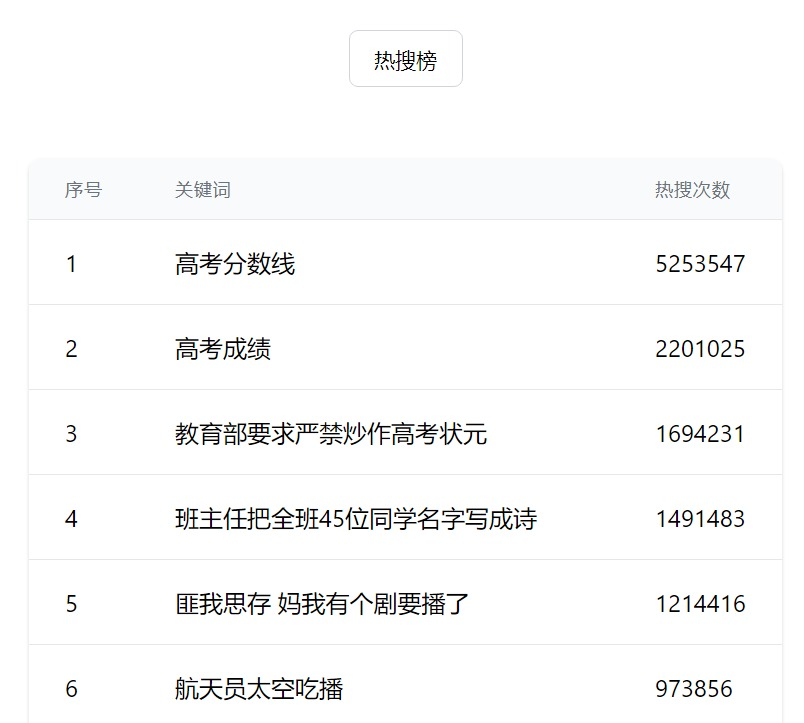
\includegraphics[width=\textwidth]{trend.jpeg}



\subsubsection{微博搜索子系统}

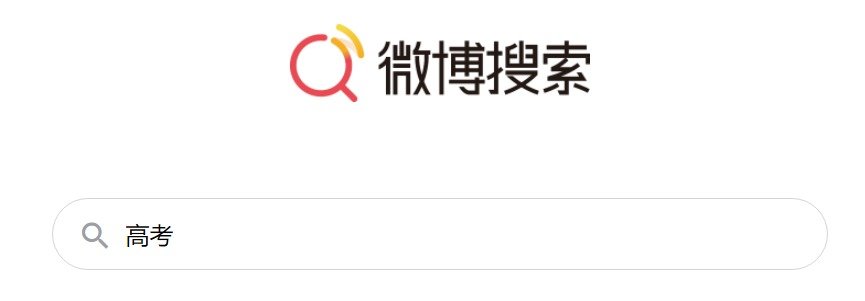
\includegraphics[width=\textwidth]{search.jpeg}


\subsubsection{微博过滤子系统}

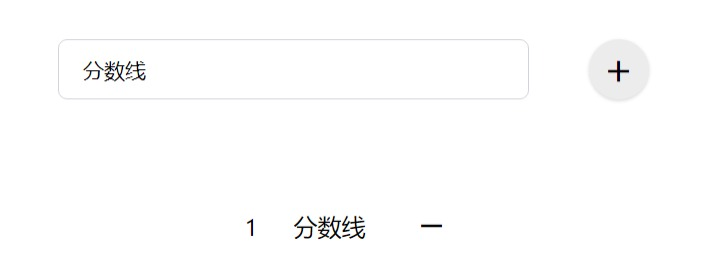
\includegraphics[width=\textwidth]{filter.jpeg}

可以查看到过滤的微博结果

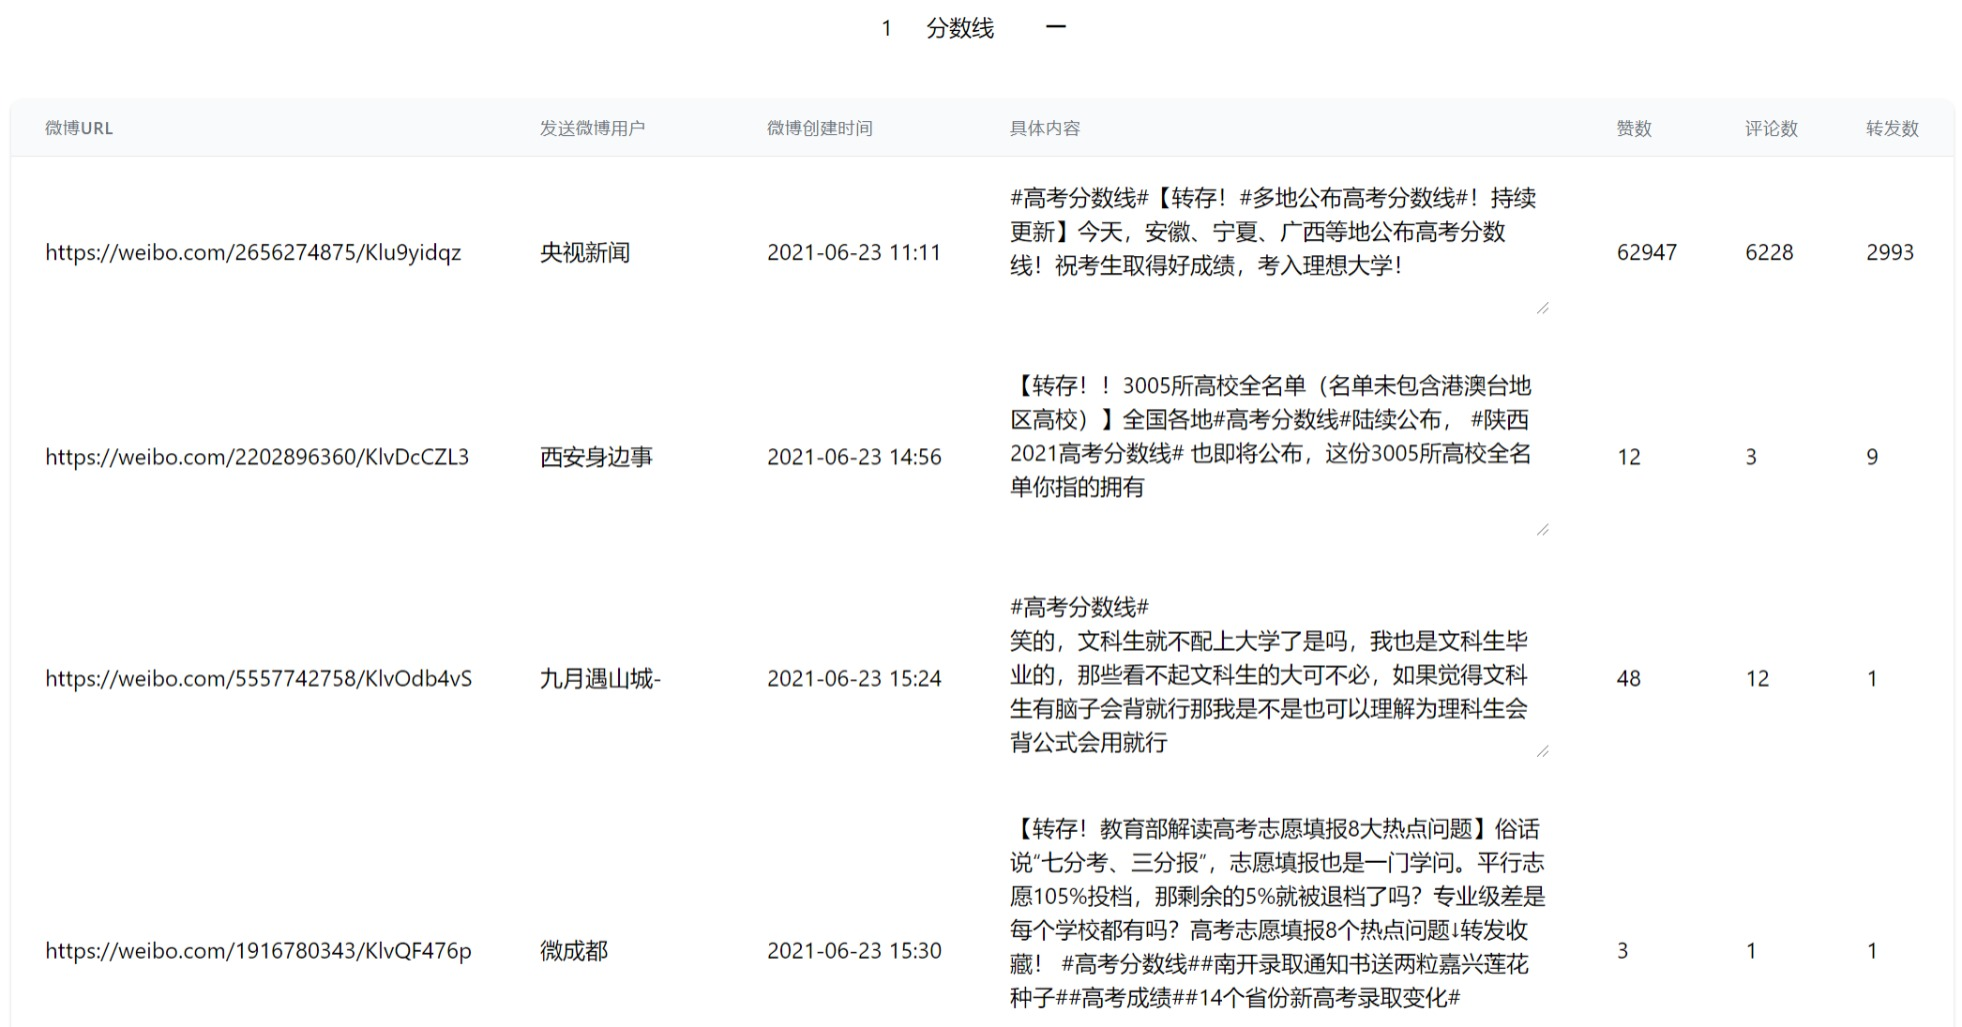
\includegraphics[width=\textwidth]{result.jpeg}

\subsubsection{微博管控子系统}
对于过滤到的微博或者特定的其他微博,可以在localhost:3000/control网站输入要管控的微博URL对该微博进行举报

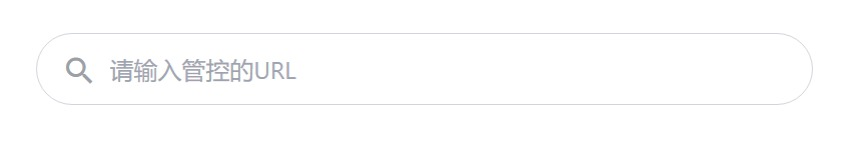
\includegraphics[width=\textwidth]{control.jpeg}
\subsubsection{数据库子系统}
在数据库子系统中,可以查看存储的热搜和微博信息

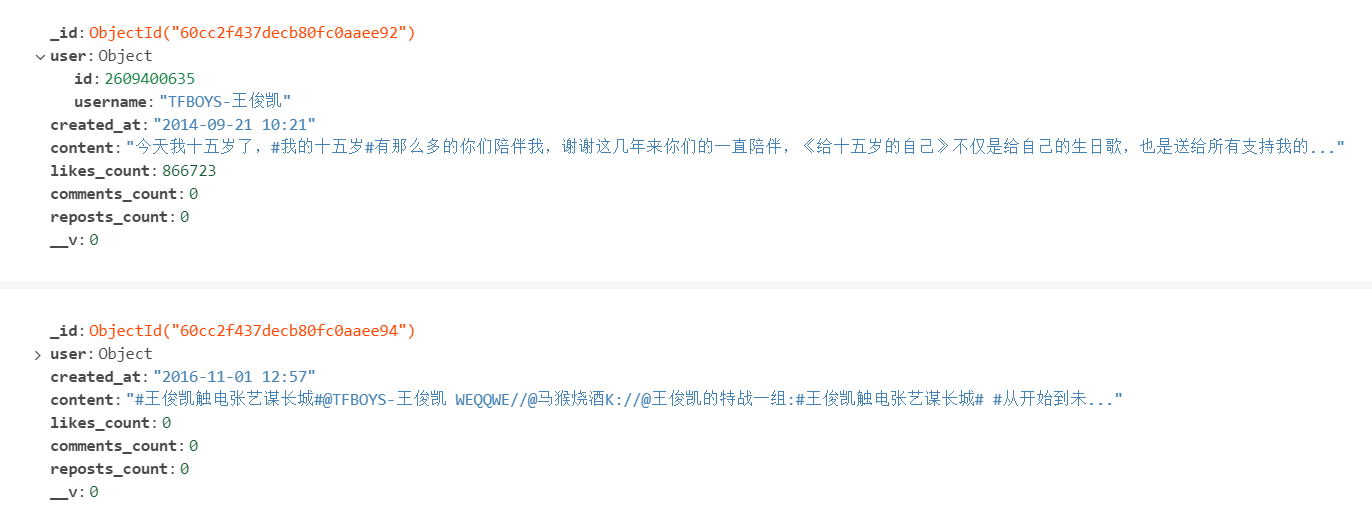
\includegraphics[width=\textwidth]{database.png}
\subsection{性能测试}

测试BF、KMP、BM算法匹配相同字符串需要的时间,结果如下:

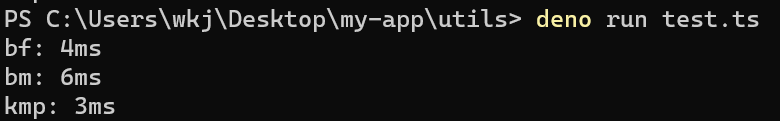
\includegraphics[width=\textwidth]{compare.png}

\section{测试总结}

\subsection{基本功能}

基本功能得到实现

\subsection{性能指标}

根据测试,实际系统中采用KMP算法作为单模式匹配,AC算法作为多模式匹配


\subsection{改进建议}
还可以采用更加先进的匹配算法,如多模式匹配的Wu-Manber算法

同时,对微博的管控需要一个登录用户,会受到单个用户举报或者发言频率的限制,也难以实现并发(需要多个账号或单个账户共享)

\end{document}